\section{GenericVcArbiter Class Reference}
\label{classGenericVcArbiter}\index{GenericVcArbiter@{GenericVcArbiter}}
{\tt \#include $<$genericVcArbiter.h$>$}

Inheritance diagram for GenericVcArbiter:\nopagebreak
\begin{figure}[H]
\begin{center}
\leavevmode
\includegraphics[height=400pt]{classGenericVcArbiter__inherit__graph}
\end{center}
\end{figure}
Collaboration diagram for GenericVcArbiter:\nopagebreak
\begin{figure}[H]
\begin{center}
\leavevmode
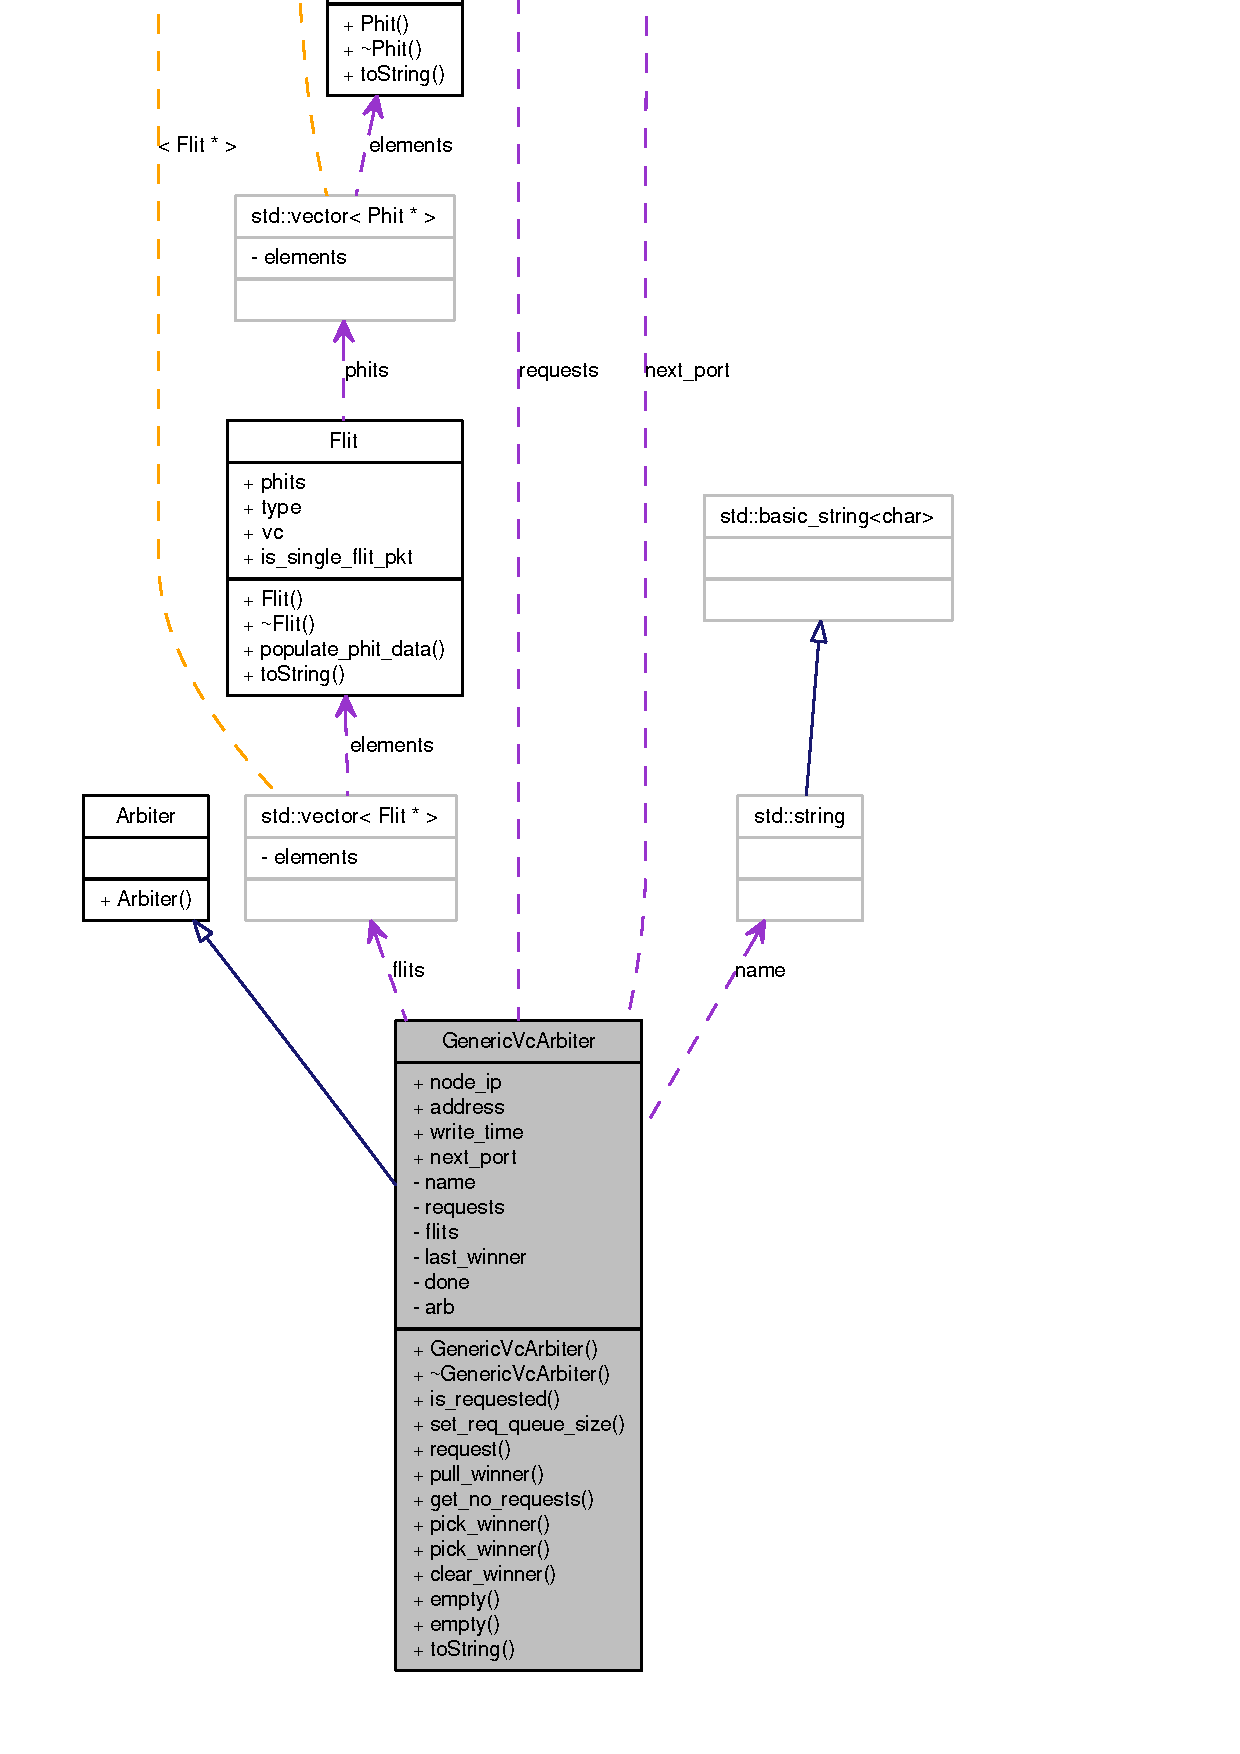
\includegraphics[width=400pt]{classGenericVcArbiter__coll__graph}
\end{center}
\end{figure}
\subsection*{Public Member Functions}
\begin{CompactItemize}
\item 
{\bf GenericVcArbiter} ()
\item 
{\bf $\sim$GenericVcArbiter} ()
\item 
bool {\bf is\_\-requested} ({\bf uint} ch)
\item 
void {\bf set\_\-req\_\-queue\_\-size} ({\bf uint} size)
\item 
void {\bf request} ({\bf Flit} $\ast$f, {\bf uint} index)
\item 
{\bf Flit} $\ast$ {\bf pull\_\-winner} ()
\item 
{\bf uint} {\bf get\_\-no\_\-requests} ()
\item 
{\bf uint} {\bf pick\_\-winner} ()
\item 
{\bf uint} {\bf pick\_\-winner} (vector$<$ bool $>$ ready)
\item 
void {\bf clear\_\-winner} ()
\item 
bool {\bf empty} ()
\item 
bool {\bf empty} (vector$<$ bool $>$ ready)
\item 
string {\bf toString} () const 
\end{CompactItemize}
\subsection*{Public Attributes}
\begin{CompactItemize}
\item 
{\bf uint} {\bf node\_\-ip}
\item 
{\bf uint} {\bf address}
\item 
unsigned long long int {\bf write\_\-time}
\item 
vector$<$ {\bf uint} $>$ {\bf next\_\-port}
\end{CompactItemize}
\subsection*{Private Attributes}
\begin{CompactItemize}
\item 
string {\bf name}
\item 
vector$<$ bool $>$ {\bf requests}
\item 
vector$<$ {\bf Flit} $\ast$ $>$ {\bf flits}
\item 
{\bf uint} {\bf last\_\-winner}
\item 
bool {\bf done}
\item 
bool {\bf arb}
\end{CompactItemize}


\subsection{Detailed Description}


Definition at line 33 of file genericVcArbiter.h.

\subsection{Constructor \& Destructor Documentation}
\index{GenericVcArbiter@{GenericVcArbiter}!GenericVcArbiter@{GenericVcArbiter}}
\index{GenericVcArbiter@{GenericVcArbiter}!GenericVcArbiter@{GenericVcArbiter}}
\subsubsection[{GenericVcArbiter}]{\setlength{\rightskip}{0pt plus 5cm}GenericVcArbiter::GenericVcArbiter ()}\label{classGenericVcArbiter_8ad20b81e2a38303b310d15e1dcc9947}




Definition at line 24 of file genericVcArbiter.cc.

References address, done, last\_\-winner, name, and node\_\-ip.\index{GenericVcArbiter@{GenericVcArbiter}!$\sim$GenericVcArbiter@{$\sim$GenericVcArbiter}}
\index{$\sim$GenericVcArbiter@{$\sim$GenericVcArbiter}!GenericVcArbiter@{GenericVcArbiter}}
\subsubsection[{$\sim$GenericVcArbiter}]{\setlength{\rightskip}{0pt plus 5cm}GenericVcArbiter::$\sim$GenericVcArbiter ()}\label{classGenericVcArbiter_da76ff9f227949f97ecd02d1bf89b5c8}




Definition at line 33 of file genericVcArbiter.cc.

\subsection{Member Function Documentation}
\index{GenericVcArbiter@{GenericVcArbiter}!clear\_\-winner@{clear\_\-winner}}
\index{clear\_\-winner@{clear\_\-winner}!GenericVcArbiter@{GenericVcArbiter}}
\subsubsection[{clear\_\-winner}]{\setlength{\rightskip}{0pt plus 5cm}void GenericVcArbiter::clear\_\-winner ()}\label{classGenericVcArbiter_4cd15ea7b1b8ff50cbd9148826880fdf}




Definition at line 164 of file genericVcArbiter.cc.

References last\_\-winner, and requests.\index{GenericVcArbiter@{GenericVcArbiter}!empty@{empty}}
\index{empty@{empty}!GenericVcArbiter@{GenericVcArbiter}}
\subsubsection[{empty}]{\setlength{\rightskip}{0pt plus 5cm}bool GenericVcArbiter::empty (vector$<$ bool $>$ {\em ready})}\label{classGenericVcArbiter_89fe4818dbc079a5305db9cfe23fd5a3}




Definition at line 185 of file genericVcArbiter.cc.

References \_\-DBG, and requests.\index{GenericVcArbiter@{GenericVcArbiter}!empty@{empty}}
\index{empty@{empty}!GenericVcArbiter@{GenericVcArbiter}}
\subsubsection[{empty}]{\setlength{\rightskip}{0pt plus 5cm}bool GenericVcArbiter::empty ()}\label{classGenericVcArbiter_c03a3978b5564acfd561a097384570d5}




Definition at line 175 of file genericVcArbiter.cc.

References requests.\index{GenericVcArbiter@{GenericVcArbiter}!get\_\-no\_\-requests@{get\_\-no\_\-requests}}
\index{get\_\-no\_\-requests@{get\_\-no\_\-requests}!GenericVcArbiter@{GenericVcArbiter}}
\subsubsection[{get\_\-no\_\-requests}]{\setlength{\rightskip}{0pt plus 5cm}{\bf uint} GenericVcArbiter::get\_\-no\_\-requests ()}\label{classGenericVcArbiter_0648f3756140fa6acc1e9345015b3461}




Definition at line 79 of file genericVcArbiter.cc.

References requests.\index{GenericVcArbiter@{GenericVcArbiter}!is\_\-requested@{is\_\-requested}}
\index{is\_\-requested@{is\_\-requested}!GenericVcArbiter@{GenericVcArbiter}}
\subsubsection[{is\_\-requested}]{\setlength{\rightskip}{0pt plus 5cm}bool GenericVcArbiter::is\_\-requested ({\bf uint} {\em ch})}\label{classGenericVcArbiter_bea0f63a51a1bfbfe7bd3a3ee0b95b48}




Definition at line 65 of file genericVcArbiter.cc.

References \_\-DBG, and requests.\index{GenericVcArbiter@{GenericVcArbiter}!pick\_\-winner@{pick\_\-winner}}
\index{pick\_\-winner@{pick\_\-winner}!GenericVcArbiter@{GenericVcArbiter}}
\subsubsection[{pick\_\-winner}]{\setlength{\rightskip}{0pt plus 5cm}{\bf uint} GenericVcArbiter::pick\_\-winner (vector$<$ bool $>$ {\em ready})}\label{classGenericVcArbiter_d5d1e1d3532c52f4e3cdb92ab2a235ec}




Definition at line 128 of file genericVcArbiter.cc.

References \_\-DBG, done, last\_\-winner, and requests.\index{GenericVcArbiter@{GenericVcArbiter}!pick\_\-winner@{pick\_\-winner}}
\index{pick\_\-winner@{pick\_\-winner}!GenericVcArbiter@{GenericVcArbiter}}
\subsubsection[{pick\_\-winner}]{\setlength{\rightskip}{0pt plus 5cm}{\bf uint} GenericVcArbiter::pick\_\-winner (void)}\label{classGenericVcArbiter_55ce40bdf8fa7c2ea448ee5aa5c50921}




Definition at line 97 of file genericVcArbiter.cc.

References \_\-DBG, done, last\_\-winner, and requests.

Referenced by pull\_\-winner().

Here is the caller graph for this function:\nopagebreak
\begin{figure}[H]
\begin{center}
\leavevmode
\includegraphics[width=186pt]{classGenericVcArbiter_55ce40bdf8fa7c2ea448ee5aa5c50921_icgraph}
\end{center}
\end{figure}
\index{GenericVcArbiter@{GenericVcArbiter}!pull\_\-winner@{pull\_\-winner}}
\index{pull\_\-winner@{pull\_\-winner}!GenericVcArbiter@{GenericVcArbiter}}
\subsubsection[{pull\_\-winner}]{\setlength{\rightskip}{0pt plus 5cm}{\bf Flit} $\ast$ GenericVcArbiter::pull\_\-winner ()}\label{classGenericVcArbiter_af615d6c6a206070c87e2ecdf82a717d}




Definition at line 47 of file genericVcArbiter.cc.

References \_\-DBG, done, flits, last\_\-winner, pick\_\-winner(), and requests.\index{GenericVcArbiter@{GenericVcArbiter}!request@{request}}
\index{request@{request}!GenericVcArbiter@{GenericVcArbiter}}
\subsubsection[{request}]{\setlength{\rightskip}{0pt plus 5cm}void GenericVcArbiter::request ({\bf Flit} $\ast$ {\em f}, \/  {\bf uint} {\em index})}\label{classGenericVcArbiter_c118c1a5cc6a9d105cd6ac5c54c7fe77}




Definition at line 39 of file genericVcArbiter.cc.

References flits, and requests.\index{GenericVcArbiter@{GenericVcArbiter}!set\_\-req\_\-queue\_\-size@{set\_\-req\_\-queue\_\-size}}
\index{set\_\-req\_\-queue\_\-size@{set\_\-req\_\-queue\_\-size}!GenericVcArbiter@{GenericVcArbiter}}
\subsubsection[{set\_\-req\_\-queue\_\-size}]{\setlength{\rightskip}{0pt plus 5cm}void GenericVcArbiter::set\_\-req\_\-queue\_\-size ({\bf uint} {\em size})}\label{classGenericVcArbiter_9424efde9588993e6b7315bd8e536ee9}




Definition at line 85 of file genericVcArbiter.cc.

References flits, next\_\-port, and requests.\index{GenericVcArbiter@{GenericVcArbiter}!toString@{toString}}
\index{toString@{toString}!GenericVcArbiter@{GenericVcArbiter}}
\subsubsection[{toString}]{\setlength{\rightskip}{0pt plus 5cm}string GenericVcArbiter::toString () const}\label{classGenericVcArbiter_b2b98c13d7e7c13e703845591f241e70}




Definition at line 202 of file genericVcArbiter.cc.

References last\_\-winner, and requests.

\subsection{Member Data Documentation}
\index{GenericVcArbiter@{GenericVcArbiter}!address@{address}}
\index{address@{address}!GenericVcArbiter@{GenericVcArbiter}}
\subsubsection[{address}]{\setlength{\rightskip}{0pt plus 5cm}{\bf uint} {\bf GenericVcArbiter::address}}\label{classGenericVcArbiter_05e08631ed998739acf72c773bfda374}




Definition at line 37 of file genericVcArbiter.h.

Referenced by GenericVcArbiter().\index{GenericVcArbiter@{GenericVcArbiter}!arb@{arb}}
\index{arb@{arb}!GenericVcArbiter@{GenericVcArbiter}}
\subsubsection[{arb}]{\setlength{\rightskip}{0pt plus 5cm}bool {\bf GenericVcArbiter::arb}\hspace{0.3cm}{\tt  [private]}}\label{classGenericVcArbiter_a0297bcb5e78e8ccfed15b025273ff9f}




Definition at line 65 of file genericVcArbiter.h.\index{GenericVcArbiter@{GenericVcArbiter}!done@{done}}
\index{done@{done}!GenericVcArbiter@{GenericVcArbiter}}
\subsubsection[{done}]{\setlength{\rightskip}{0pt plus 5cm}bool {\bf GenericVcArbiter::done}\hspace{0.3cm}{\tt  [private]}}\label{classGenericVcArbiter_6d5b07856fdfec01e2a11966733f97e6}




Definition at line 64 of file genericVcArbiter.h.

Referenced by GenericVcArbiter(), pick\_\-winner(), and pull\_\-winner().\index{GenericVcArbiter@{GenericVcArbiter}!flits@{flits}}
\index{flits@{flits}!GenericVcArbiter@{GenericVcArbiter}}
\subsubsection[{flits}]{\setlength{\rightskip}{0pt plus 5cm}vector$<${\bf Flit}$\ast$ $>$ {\bf GenericVcArbiter::flits}\hspace{0.3cm}{\tt  [private]}}\label{classGenericVcArbiter_d1e2667bb1e9dff025910f9f5f1234f9}




Definition at line 62 of file genericVcArbiter.h.

Referenced by pull\_\-winner(), request(), and set\_\-req\_\-queue\_\-size().\index{GenericVcArbiter@{GenericVcArbiter}!last\_\-winner@{last\_\-winner}}
\index{last\_\-winner@{last\_\-winner}!GenericVcArbiter@{GenericVcArbiter}}
\subsubsection[{last\_\-winner}]{\setlength{\rightskip}{0pt plus 5cm}{\bf uint} {\bf GenericVcArbiter::last\_\-winner}\hspace{0.3cm}{\tt  [private]}}\label{classGenericVcArbiter_9b5188dbe90faf50fa08d2589930124d}




Definition at line 63 of file genericVcArbiter.h.

Referenced by clear\_\-winner(), GenericVcArbiter(), pick\_\-winner(), pull\_\-winner(), and toString().\index{GenericVcArbiter@{GenericVcArbiter}!name@{name}}
\index{name@{name}!GenericVcArbiter@{GenericVcArbiter}}
\subsubsection[{name}]{\setlength{\rightskip}{0pt plus 5cm}string {\bf GenericVcArbiter::name}\hspace{0.3cm}{\tt  [private]}}\label{classGenericVcArbiter_f2dcce4276d8321619178efac8f00aa5}




Definition at line 60 of file genericVcArbiter.h.

Referenced by GenericVcArbiter().\index{GenericVcArbiter@{GenericVcArbiter}!next\_\-port@{next\_\-port}}
\index{next\_\-port@{next\_\-port}!GenericVcArbiter@{GenericVcArbiter}}
\subsubsection[{next\_\-port}]{\setlength{\rightskip}{0pt plus 5cm}vector$<${\bf uint} $>$ {\bf GenericVcArbiter::next\_\-port}}\label{classGenericVcArbiter_1538dd58584a6130c0846fa7da7a376d}




Definition at line 55 of file genericVcArbiter.h.

Referenced by set\_\-req\_\-queue\_\-size().\index{GenericVcArbiter@{GenericVcArbiter}!node\_\-ip@{node\_\-ip}}
\index{node\_\-ip@{node\_\-ip}!GenericVcArbiter@{GenericVcArbiter}}
\subsubsection[{node\_\-ip}]{\setlength{\rightskip}{0pt plus 5cm}{\bf uint} {\bf GenericVcArbiter::node\_\-ip}}\label{classGenericVcArbiter_f5fe6167805ebb6bda85e58535b6f51e}




Definition at line 36 of file genericVcArbiter.h.

Referenced by GenericVcArbiter().\index{GenericVcArbiter@{GenericVcArbiter}!requests@{requests}}
\index{requests@{requests}!GenericVcArbiter@{GenericVcArbiter}}
\subsubsection[{requests}]{\setlength{\rightskip}{0pt plus 5cm}vector$<$bool$>$ {\bf GenericVcArbiter::requests}\hspace{0.3cm}{\tt  [private]}}\label{classGenericVcArbiter_dd5c93221687ab6778e467366f75e845}




Definition at line 61 of file genericVcArbiter.h.

Referenced by clear\_\-winner(), empty(), get\_\-no\_\-requests(), is\_\-requested(), pick\_\-winner(), pull\_\-winner(), request(), set\_\-req\_\-queue\_\-size(), and toString().\index{GenericVcArbiter@{GenericVcArbiter}!write\_\-time@{write\_\-time}}
\index{write\_\-time@{write\_\-time}!GenericVcArbiter@{GenericVcArbiter}}
\subsubsection[{write\_\-time}]{\setlength{\rightskip}{0pt plus 5cm}unsigned long long int {\bf GenericVcArbiter::write\_\-time}}\label{classGenericVcArbiter_92c6b36810e3ca21255596f2fde60a96}




Definition at line 50 of file genericVcArbiter.h.

The documentation for this class was generated from the following files:\begin{CompactItemize}
\item 
{\bf genericVcArbiter.h}\item 
{\bf genericVcArbiter.cc}\end{CompactItemize}
